\documentclass {article}[a4paper,12pt]

\usepackage[ngerman]{babel} % Deutsch ngerman -> neue Rechtschreibung
\usepackage[utf8]{inputenc}
\usepackage[T1]{fontenc}
\usepackage{csquotes}       % Anführungszeichen
\usepackage[hidelinks]{hyperref}
\usepackage{graphicx}
\usepackage{graphics}
\usepackage{titlesec}
\usepackage{blindtext}
\usepackage{pdfpages}
\usepackage{amsmath}
\usepackage{amssymb}


\title {Dokumentation: RNKS Beleg}
\date{ws23/24}
\author{A.Gröber | s80438}

\begin{document}
\maketitle
\newpage
\tableofcontents
\newpage
\section{Dokumentation und  Lernportfolie (Aufgaben 1-7)}

Das Folgende Segment dient als Lernportfolie für die Programmieraufgaben 1-7
\subsection {Aufgaben 1 und 2}

Wie im Screencast gezeigt implementiert. Fenstergröße erstmal auf 1 lassen. Ich versuche erstmal nur stop and wait
zu programmieren.
\subsection{Vorbereitung auf 3}
SW-Diagramme erstellt (im Diagramm Ordner zu finden).
\newpage
\begin{figure}
\newpage
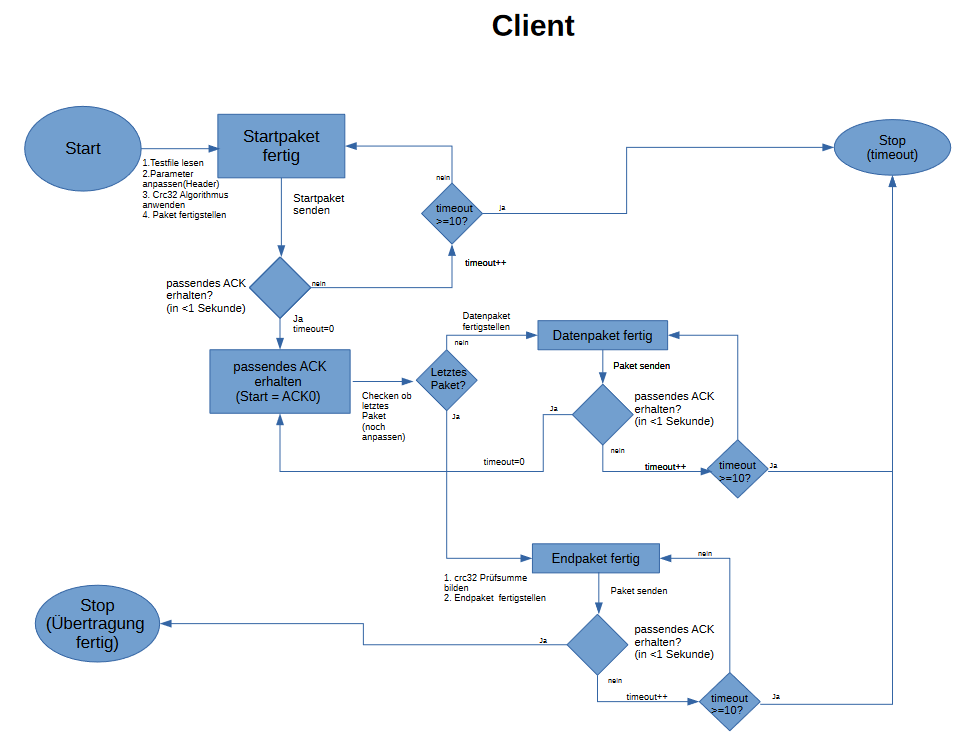
\includegraphics[width=0.6\linewidth]{Diagramme/Client.png}
\caption{Client}
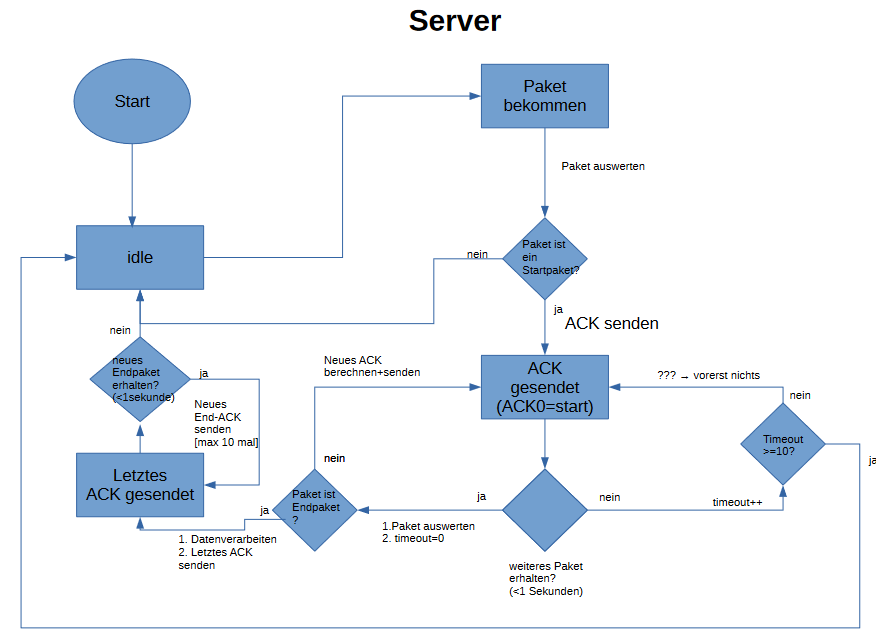
\includegraphics[width=0.6\linewidth]{Diagramme/Server.png}
\caption{Server}
\end{figure}
\newpage



\subsection{Aufgabe 3 Erste Schritte}

Ich habe sehr lange gebraucht um die Klassen und deren Funktionalität etwas zu verstehen,
habe es aber geschafft eine Testdatei zu übertragen (ein Datenpaket nach empfangen des ACK0 zu schicken welches selbst auf kein
ACK wartet) nächster Schritt ist eine Größere Datei zu verschicken und dieses in einzelne Pakete zu teilen möglicherweise
schon ACK's berücksichtigen. Zudem stellt sich die Frage ob einzelene Pakete direkt an die Datei angehängt werden oder erst
in einen Puffer oder Tmpdatei (zwischenspeicher) und dann gesammelt in die Datei übertragen werden, was passiert hier wenn Paket fehlerhaft ist?.
\newline
Probleme: 
\newline
ACK wird nicht berücksichtigt
\newline
Noch keine Pakete 	---> nächster Schritte vor  Aufgabe 4
\newline  \newline
Fortschritt: 
\newline
make.sh+Methode: WriteToFile()

\subsection{Aufgabe 3/5 Pakete bauen/auf ACKs warten}
Mithilfe von Bytebuffern und deren funktionen [allocate,put*], Startpaket gepackt und abgeschickt.
Erstmal in eine Testdatei gespeichert ---> alle daten kammen in gewünschter form an.
Struktur  für  Datenpakete + Endpakete erstellt nach selben Schema.
\newline
nächster Schritt:
Struktur zum Antworten bzw. warten der Acks, (später Timeout Bedingungen und  Aufgabe 4)
\newline
Fortschritt: Paketstrukturen und erste  "Verarbeitung  eines  Pakets".
\newline
Probleme: wenig Verständis für die Methoden/Funktionen in der Klasse SW
\newline
----------------------------------------------------------------------------------------------------
\newline
Ich habe ein bisschen mit den Funktionen in SW herumprobiert und
erstmal simple Acks (nur ACK:packNr) zurückgegeben.
Timeouts noch nicht gesetzt außer in der waitforAck funktion.
Startpacket komplett gesendet und empfangen+ausgewertet und die CRC32 summen verglichen.
Daraufhin Datei geöffnet und test String darin abgelegt. Dies hat  auf localhost ohne Packetverlust  funktioniert.
\newline
nächster Schritt: 
\newline
1. Datenpackete auswerten (in angelegte Datei schreiben) und Acks nach Protokoll verschicken+verabeiten
   +Endpacket identifizieren und verarbeiten
\newline
2. Timouts setzen
\newline
3. wenn möglich den Server/Port "reseten", sodass mehrere clients nacheinander dateiene senden können.
\newline
4. auf Kanal mit delay und fehlerrate testen.
\newline
Fortschritt: Vollständige Struktur beim Sender, beim Server fehlt die  verarbeitung des Endpakets  und rückgabe vollständiger Acks
\newline
----------------------------------------------------------------------------------------------------
\newline
Acks wie im Protokoll vorgesehen implementiert außer für letztes Paket.
\newline
Problem: wie unterscheidet Server  letztes Paket von einen normalen daten Paket,
provisorische Lösung End-PacketNr=127 senden.
\newline
----------------------------------------------------------------------------------------------------
\newline
Auf localhost große Datei verschickt diese mittels crc32-summen gecheckt, diese wird jetzt
Fehlerlos in das Verzeichnis Upload/ kopiert.
Allerdings funktionieren nur Dateiformate die keine Nullbytes enthalten (Text funktioniert, png nicht),
Da Ich mittels der Funktion filterNullbytes überschüßige Nullbytes von der Request entferne (falls das Dateiformat diese enthält, wird das Paket nur bis zur Stelle des ersten Nullbytes nach der Paketnr eingelesen)
\newline
Workarounds:Paketnr letztes Paket=127 | nur bestimmte Formate erlaubt
\newline
nächster Schritt: EndAck implementieren, Timeouts einfügen, Workarounds bearbeiten wenn mögl.
\newline
Fortschritt: Datei senden ohne fehler möglich, crc32 summen stimmen für  startpaket sowie für ganze datei überein.
Server kann mehrere Dateien hinteinander empfangen.
\newline
---------------------------------------------------------------------------------------------------
\newline
Keine Lösung für das Problem mit dem letzten Paket zur Unterscheidung  vom normalen Daten-Paket,
daher ist das letzte Paket mit PaketNr 127 gekenzeichnt (sowie das entsprechende Ack=FAck).
Ganze Datei wird  jetzt übertragen und FAck kommt wie gewünscht an mit richtigem CRC32 Wert.
\newline
nächster Schritt: Timeouts --> auf channel mit fehlern testen
\newline
----------------------------------------------------------------------------------------------------
\newline
Timeouts fertig, auf localhost ist eine Datei übertragung mit fehlerbehaftetem Kanalmöglich (Testszenario: 10KB=10DP+1SP+1FP mit bis zu 0.5 fehlerrate und 200ms delay)
\newline
nächster Schritt: Aufgabe 4
\newline
----------------------------------------------------------------------------------------------------
\newline
test logger auskommentiert, Datenraten mittels System.currentTimeMillis() und Datasize bzw. Filesize implementiert
\newline
nächster Schritt: Mit VPN auf hochschulservern testen.
\newline
1.Abgabe hier
\subsection{Änderungen von 1. Abgabeversion zur aktuellen}
Client: letztes Datenpaket von Endpaket getrennt (Endpacket jetzt nur 7Byte)
\newline
Das hat auch auf dem Hochschulserver Funktioniert
\newline
Server: Eigentliches Paket (max 1027Byte) aus dem vom Socket gesendeten Paket (65555Byte [null]) extrahieren. Neue Struktur zum verarbeiten
\newline
Jedes Dateiformat und beliebig viele Datenpackete können gesendet werden. Lokal sowie auf Hochschulserver.
\newline
Server weiter angepasst und 60 Sekunden Timeout hinzugefügt,CloseConnection eingefügt.
\newline
1 Workaround/Probleme:
\newline
1. Um normales Datenpaket von letztem Datenpaket voneinander zu unterscheiden, wird die Größe des Pakets mit einer Variable verglichen.
Die globale Variable datasize-check gibt die zu vergleichende Größe für das 1.DP an und sollte so groß sein wie Datasize (Datenanteil im Datenpaket vom Client).
Das ist unsauber gelöst und funktioniert nur wenn Datasize>=datasize-check.
\newpage
\section{Aufgabe 8: Theorieaufgabe}


\href{https://de.wikipedia.org/wiki/Datendurchsatz}{Ethernetgeschwindigkeit-link}
\newline
Grundlage der Rechnung im Bsp der Sicherungsschicht abgehandelt.
\newline
\newline
L=1400Byte+3Byte (Seasionnummer+Paketnummer) gerundet 1400
Start+Endpaket sind kleiner daher vernachlässigbar in der Rechnung
\newline
\newline
\textit{geg.:} 
\\
$ L = 1.400 \text{ Byte } = 11.200 \text{ Bit } $ \\
$ T_w = 0,01 \text{ s } $ \\
$ P_e = P_r = 0,1 $  \\
$ R = 1 $ \\ 
\\
\textit{ges.:}
\\
$ \eta_{sw} $ \\ 
$ \eta_{sw} = \frac{T_p}{T_{p} + T_{w}}(1-P_{e})(1-P_{r})*R $  \\
\\
\textit{lsg.:} 
\\
$ T_p = \frac{L}{r_b} = \frac{11.200 \text{ Bit}}{ 94/2\text{ MBit/s}} = 0.00024 \text{s} $ \\
\\ohne fehler: \\
\\
$ \eta_{sw}  = \frac{0,00024\text{ s }}{{0,00024}\text{s}+0.01\text{s}}$ \\
\\
$ \eta_{sw}  = 0.023$ \\
\\ Symbolfehlerrate mit eigentlichen Datendurchsatz multiplizieren\\
\\
$ 0.023 * 94/2\text{ MBit/s } = 1.081 \text{ MBit/s} $ \\ 
$ 1.081 \text{ MBit/s} * 1000 = 1081 \text{ Kbit/s} $ \\ 
$ 930,6 \text{ Kbit/s} \div 8 = 135.125 \text{ KB/s} $ \\ 
\\
\\mit fehler \\
\\
$ \eta_{sw}  = \frac{0,00024\text{ s }}{{0,00024}\text{s}+0.01\text{s}}*0.9*0.9*1$ \\
\\
$ \eta_{sw}  = 0.018 $ \\
\\
\\ Symbolfehlerrate mit eigentlichen Datendurchsatz multiplizieren\\
\\
$ 0,0198 * 94/2\text{ MBit/s } = 0.9306 \text{ MBit/s} $ \\ 
$ 0.9306 \text{ MBit/s} * 1000 = 930,6 \text{ Kbit/s} $ \\ 
$ 930,6 \text{ Kbit/s} \div 8 = 116,325 \text{ KB/s} $ \\ 
\\
\newline
Info: Ich habe ein Kbyte als 1000 byte (bzw. 1Mbyte als 1000Kbyte) angenommen, in der Realität sind es 1024!
Das vereinfacht die Rechnung und ist nicht wirklich auschlagebend auf das Ergebnis.
\newline
\newline
Warum ist Praktische Anwendung (Beleg) langsamer?
\newline
Auf meinem Localhost komme ich mit genannten Kanalparametern auf eine Datenrate von etwa 30-60 Kbit/s. (das stimmt etwa mit dem Hochschulserver überrein)
Das lässt sich zum einen durch die relativ langen Timeouts erklären zum anderen ist meine Packetgröße nur
1024 Byte was einen maximalen Datendurchsatz von etwa 80 KB/s zulässt. Am stärksten fallen allerdings die Timeouts ins Gewicht.
\newline
Bearbeitungs bzw. Berechnungszeit der Pakete fallen aus dem Gewicht da diese sehr klein sind.
Ausgenommen von den Crc32-checks im StartPaket und letzten Ack.

\newpage
\section{Aufgabe 9: Funktionalität}

\subsection{grober Progarmmablauf}
Server und Client können seperat gestartet werden. Im Fall das der Server/Port nicht bereitsteht
wird der Client nach 10 Sekunden geschlossen. 
\newline
Der Server wartet bis zu 5 Minuten auf ein Paket bevor er die Verbindung schließt.  
Es ist möglich mehrere Client nacheinander auf dem selben Port zu bediennen.
\newline
Der Client verschickt einzelne Pakete, diese werden in der Klasse Filetransfer erstellt und mittels der Funktion
myARQ.data-req in die Klasse SW übergeben. Wo Sie zum Teil ausgelesen werden, um zu bestimmen welches Paket verschickt wird.
\newline
Innerhalb von data-req (SW-Klasse) wird das Paket über den Socket verschickt und auf eine Antwort (ACK) gewartet.
\newline
\newline
Auf Server Seite wird der Socket permanent abgehört bis ein Paket eintrifft, falls es ein Startpaket ist 
wird eine Session geöffnet (konkret wird eine Datei mit dem übergebenen Dateinamen und der Dateigröße geöffnet und ein paar globale Variablen gesetzt).
\newline
Im Fall eines  Datenpakets werden die Daten des Pakets hinten an die Datei angehängt,
selbiges gilt für das letzte Datenpaket.
\newline 
Falls ein Ack oder Paket verloren geht, wird es bis zu 10 mal erneut gesendet.
\newline
Um ein neues Ack zu erzeugen (für ein bereits bekanntes Paket), checkt die Funktion SW.data-ind-req ob Sie 
bereits ein Startpaket erhalten hat bzw. die Paketnummer.
Im Fall, dass das Paket bereits bearbeitet wurde sendet die Funktion nur ein "Ack"-String an den Server.
\newline
Die Verbindung zum Client und der Clint an sich, wird sobald das letzte Ack (FAck) eingetroffen ist, geschlossen.
Es wird auf der Konsole ausgegeben ob beide CRC32-Summen gleich sind
\newline

\subsection{Infos zur  implementierung}

1. Ich habe die Größe des Datenteils beim Datenpaket auf 1024bytes=1Kbyte festgelegt.
Diese kann mit der Variable Datasize angepasst werden.
\newline
2. Bei der Konvertierung der CRC32-Summe (long zu int) im Startpaket wird  die Summe negativ, 
das verursacht hier erstmal keine Probleme sollte aber möglicherweise angepasst  werden.
[Idee hierfür: int mit max value initialisieren und dann die CRC32 summe davon subtrahieren].
\newline
3. Pakete sind so implementiert wie es da Protokoll vorsieht.
\newline
4. Es ist nur das Stop and Wait Protokoll implementiert.
\newline

\subsection{Probleme und Limitierungen}

Timeouts sind immer 1 Sekunde was sich auf den Datendurchsatz auswirkt (im Fall das Pakete verloren gehen).
Eine bessere Strategie  wäre  vielleicht den ersten Timeout kurz zu wählen (timeout 1: 200ms),
und mit voranschreitenden Timouts, längere Timeout zeiten zu wählen (Timeout 2: 300ms usw.)
\newline
\subsection{Verbesserungsvorschläge}
- dynamische Timeouts            (Protokoll bzw.Aufgabenstellung)
\newline
- positive CRC32-Summe im Header (meine Implementation)
\newline
- andere Lösung für  letztes  Datenpaket (meine Implementation)
\newline
- Verbesserte Serverstruktur (meine Implementation)
 
\section{Verwendete Editoren,Tutorials,etc.}

\subsection{Editoren}
JDK: openjdk 11.0.21 2023-10-17
\newline
IntelliJ IDEA (Programmieren+debugen)
\newline
VS-Code (Programmieren+Latexdokumentation)
\newline
libreoffice draw (erstellen der Diagramme)

\subsection{Tutorials Java}
\href{https://www.w3schools.com/java/java_type_casting.asp}{w3 type-casting + andere Tutorials}
\newline
\href{https://stackoverflow.com/questions/6255768/java-how-create-a-package-with-bytes}{overflow bytebuffer kurz}
\newline
\href{https://stackoverflow.com/questions/9578639/best-way-to-convert-a-signed-integer-to-an-unsigned-long}{overflow java int zu long}
\newline
\href{https://docs.oracle.com/javase/8/docs/api/java/util/zip/Checksum.html}{crc32-java}
\newline
\href{https://kryptografie.de/kryptografie/chiffre/crc-32.htm}{crc-allg}
\newline
\href{https://stackoverflow.com/questions/9854166/declaring-an-unsigned-int-in-java}{unsigned int java}
\newline
\href{https://www.java-blog-buch.de/11-02-mathematisches-mit-java-lang-math/}{aufrunden genutzt in Datenpaket berechnung}
\subsection{Tutorials Latex}
\url{https://www.overleaf.com/learn/latex/Hyperlinks}
\newline
\url{https://en.wikibooks.org/wiki/LaTeX/Title_Creation}
\newline
\url{https://www.namsu.de/Extra/pakete/Graphicx.html}
\newline
\href{https://www.youtube.com/watch?v=R6etJS4XXPM&list=PL0FqMC_xCtjTg5XgHXhNPUJNib6gW_Zpi&index=3&ab_channel=ThomasErben-TutorialsundLehrvideos}
{Youtube-Playlist hauptsächlich Part3}




\end{document}
